% =====================================================================
%  Robustness paragraph + figure for app:growth  (EmergingXOR)
%  Drop the figure where you like inside app:growth and the paragraph
%  after the developmental-window paragraph.  Figure file: robustness_sweep_en.png
% =====================================================================

\begin{figure}[h]
\centering
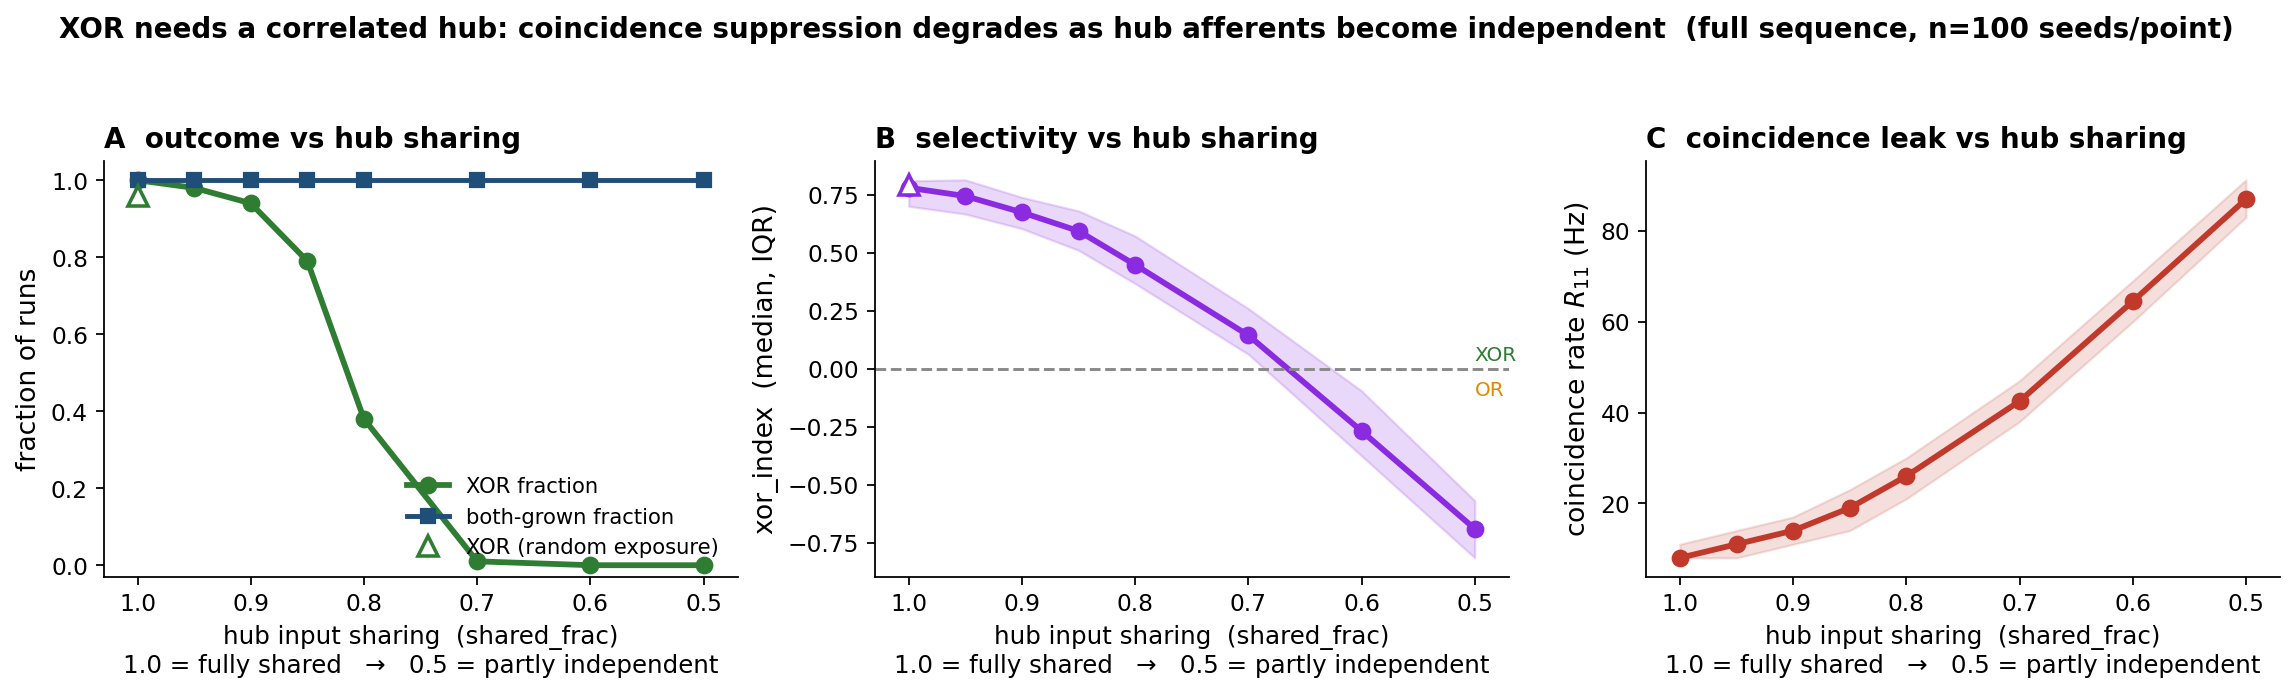
\includegraphics[width=\linewidth]{robustness_sweep_en.png}
\caption{\textbf{XOR requires a correlated hub (Brian2, 100 seeds per point).} As the
fraction of \emph{shared} afferent drive to the 20 hub cells falls from 1.0 (all hubs
see the same two Poisson trains) toward 0.5 (each hub also receives its own independent,
pattern-driven train), coincidence suppression degrades smoothly. \textbf{(A)} the fraction
of runs classified XOR falls from $1.00$ through a knee near $\mathrm{shared}\!\approx\!0.82$,
while the fraction in which \emph{both} direct arms grew stays at $1.00$ throughout.
\textbf{(B)} the continuous selectivity index
$\mathrm{xor\_index}=(\min(R_{10},R_{01})-R_{11})/\min(R_{10},R_{01})$
(median, IQR band) declines monotonically and crosses zero (XOR$\to$OR) near
$\mathrm{shared}\!\approx\!0.66$. \textbf{(C)} the coincidence read-out rate $R_{11}$ rises
from ${\sim}8$ to ${\sim}87$~Hz. Open triangles: a fully-random (unbalanced) pattern-exposure
control at $\mathrm{shared}=1.0$ (XOR $0.96$), confirming the result does not depend on
balanced exposure.}
\label{fig:robust}
\end{figure}

\paragraph{Robustness across seeds, and the role of hub correlation.}
Because a single run cannot support a developmental-learning claim, we repeated the full
sequence over $100$ random seeds and classified \emph{each} run individually
(Fig.~\ref{fig:robust}). With the shared-input hub the outcome is effectively deterministic:
XOR in $100/100$ runs, both arms grown in $100/100$, median $\mathrm{xor\_index}=0.78$
(IQR $[0.70,0.81]$), coincidence held to $R_{11}=8$~Hz (IQR $[8,11]$) against single-input
rates of ${\sim}41$~Hz. A fully-random (unbalanced) pattern-exposure control is essentially
identical (XOR $96/100$; the four exceptions are borderline sub-threshold single-input rates
that remain XOR-like by the continuous index), so the result is not an artefact of balanced
exposure. The one manipulation that does matter is the correlation of the hub's afferents:
when each hub cell receives a mixture of the shared trains and its own independent,
pattern-driven train, coincidence suppression degrades smoothly as sharing is reduced ---
$R_{11}$ rises monotonically ($8\to87$~Hz), $\mathrm{xor\_index}$ falls and crosses zero near
$\mathrm{shared}\!\approx\!0.66$, and the XOR fraction drops through a knee near $0.82$,
becoming OR by $\mathrm{shared}\!\lesssim\!0.6$. Crucially, \emph{both arms grow in $100\%$ of
runs across the entire sweep}: what fails as the hub de-correlates is not the growth of the
direct arms but the coincidence-dependent shunt.

This sharpens what the model does and does not show. The plasticity rule does not discover the
XOR architecture; that architecture is preconfigured --- both inputs converging on the hub, the
hub's supralinear threshold, the hub projecting to both laterals, the read-out pooling both
laterals, and mature GABA becoming shunting. What the two-phase sequence contributes is
developmental: the depolarizing \emph{builder} lifts otherwise-subthreshold arms into a
functional regime, and the switch then lets the same pre-positioned hub express coincidence
suppression --- \emph{provided} that suppression rests on the synchronous recruitment of a
correlated hub population. In this reading the GABA switch \emph{matures} a preconfigured
XOR scaffold rather than carving XOR \emph{de novo}.
